%  Created by Branden Stone on 2015-01-15.
%  Copyright (c) 2015 Branden Stone. All rights reserved.
%--------------------------------------------------------
\documentclass{article}


%---------------------------
% Packages
%---------------------------
\usepackage{amssymb, amsmath, latexsym, amsfonts, amsthm, mathrsfs} % Standard packages that are nice to have.
\usepackage{amsrefs} % Allows for easy referencing and citations.
\usepackage{verbatim} % Needed for \begin{comment} \end{comment}.
\usepackage[text={6in,9in},centering]{geometry} % Defines the dimensions of the text body.
\usepackage[colorlinks=true]{hyperref} % Allows for use of hyperlinks.
%\usepackage[doublespacing]{setspace} % Makes the document double spaced.
\usepackage[pdftex]{graphicx} % Allows for \includegraphics
\usepackage{enumerate} % Allows for easy modification of lists

\renewcommand{\arraystretch}{1.5}

%----------------------------
% Title and Author
%----------------------------

\title{Math 390 Homework 7}
\author{Due Friday, March 25}
\date{}


%----------------------------
% Main Document Body
%----------------------------

\begin{document}


%-------------------------------------------------------------
% Front Matter: This is where you can add a table of contents,
% preface, list of figures, ETC. for this template we will 
% only create a title and author name with `\maketitle'
%-------------------------------------------------------------

\maketitle

\setlength{\parindent}{0em} % Sets indentation of new paragraph
\setlength{\parskip}{1em} % Sets space between paragraphs

%-------------------------------------------------------------
% Document Body: Essentially this is where you place the 
% content of your document. To use this template, just delete
% all of the text between here and the Bibliography Section.
% Then type whatever you desire.
%-------------------------------------------------------------


Solutions should be written \LaTeX\ or Markdown and converted to a PDF. You are encouraged to work with others
on the assignment, but you should write up your own solutions independently. This means no copy pasting. You should
reference all of your sources, including your collaborators. 

\begin{enumerate}

\item Determine the number of labeled spanning trees of the Petersen graph. (Hint: Use the Matrix Tree Theorem, Theorem 10.3 in Edition 4 and Theorem 3.5 in Edition 5. I recommend using a computer to compute the determinant.)

\item 
\begin{enumerate}
	\item Read the definition of the {\it chromatic number} (5th edition p. 101, 4th edition p. 81). The Four Color Theorem (Thm 5.5/Thm 17.5) says that every simple planar graph is 4-colorable. Give an example of a planar graph whose chromatic number is 4.
	
	\item A graph is {\it outerplanar} if it has a planar drawing with all the vertices lying on the outside face. Use the Four Color Theorem to show that the chromatic number of an outerplanar graph is at most three. (Hint: Add a vertex to the outside face with edges to all the other vertices.)
\end{enumerate}

\item \begin{enumerate}
	\item Use Kuratowski's Theorem to show that $K_{2,3}$ and $K_4$ are not outerplanar.

	\item Use Kuratowski's Theorem to show that a graph is outerplanar if and only if it does not contain a subgraph homeomorphic to $K_{2,3}$ or $K_4$.

	\item For each of the following graphs, determine if the graph is outerplanar. If the graph is outerplanar, show a planar drawing with all the vertices lying on the outside face. If the graph is not outerplanar, show that it contains a subgraph homeomorphic to $K_{2,3}$ or $K_4$.
\end{enumerate}

\begin{center}
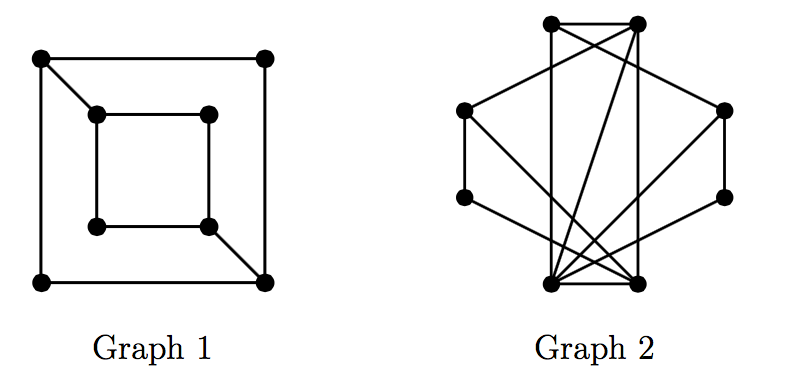
\includegraphics[width=.5\textwidth]{pic1.png}	
\end{center}


\item A graph has genus $g$ if the graph can be drawn on a $g$-holed-torus without edge crossings but cannot be drawn on a $(g-1)$-holed-torus without edge crossings. The genus of a graph $G$ is denoted $g(G)$.

\begin{enumerate}
	\item  Determine the genus of $K_{3,5}$.
	\item Show that $g(K_{r,s}) \geqslant \frac 1 4 (r - 2)(s - 2)$. ({\it Hint:} Recall that for graphs drawn on a $g$-holed-torus, $n-m+f = 2 -2g$.)
\end{enumerate}

\pagebreak

\item For each of the following graphs, determine the chromatic number of the graph, and show a coloring that uses the minimum number of colors. (You do not need to prove that your answer is a minimum.)
\begin{center}
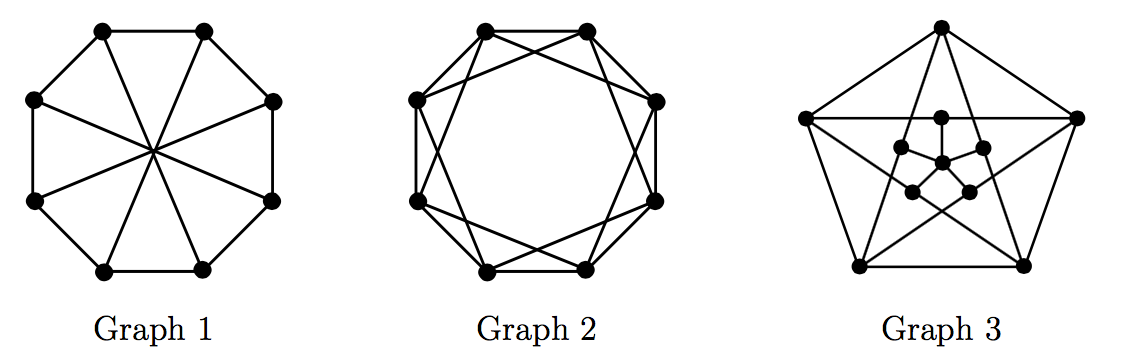
\includegraphics[width=.8\textwidth]{pic2.png}	
\end{center}


\end{enumerate}




\end{document}